\section{Fuzzy logic}

Fuzzy logic is an infinite-valued logic with truth values ranging from 0 to 1, where propositions are expressed in the form of "A is L," where:
\begin{itemize}
    \item A is a linguistic variable.
    \item L is a label representing a fuzzy set.
\end{itemize}
Formally, a linguistic variable is defined by a 5-tuple (X, T(X), U, G, M), where: 
\begin{itemize}
    \item X is the name of the variable.
    \item T(X) is the set of term for X, each corresponding to a fuzzy variable denoted by T(X) and ranging on U.
    \item U is the universe of discourse defined on a base variable u.
    \item G is the syntactic rule used to generate the interpretation X of each value u.
    \item M is the semantic rule used to associate to X its meaning.
\end{itemize}
\begin{example}
    Let's define a linguistic variable for age as follows:
    \begin{itemize}
        \item X is a linguistic variable labelled "age".
        \item $\textnormal{U}=[0,100]$.
        \item $\textnormal{T(X)}=\{old, middle-aged, young, \dots\}$.
        \item $\textnormal{u}=[0,+\infty]$.
        \item M represents the definition in terms of fuzzy sets for the values of X.
        \item G is responsible for the fuzzy matching interpretation of u.
    \end{itemize}
\end{example}
Now that we have defined the linguistic variable, it is possible to express a simple proposition as "p: X is F", where:
\begin{itemize}
    \item X is a linguistic variable.
    \item F is the label of a fuzzy set defined on U, representing a fuzzy predicate.
    \item $\mu_{\textnormal{F(x)}}$ is the membership function defining F, and it is interpreted as the truth value for the proposition p ($\textnormal{T(p)}=\mu_{\textnormal{F(x)}}$).
\end{itemize}
Hence, the truth value of the proposition P is a fuzzy set defined on the interval $[0,1]$.
\begin{example}
    Consider the simple proposition "p: temperature is high", with X representing temperature and F representing high. 
    We can determine the truth value of this proposition using the graph of the membership function as shown below:        
    \begin{figure}[H]
        \centering
        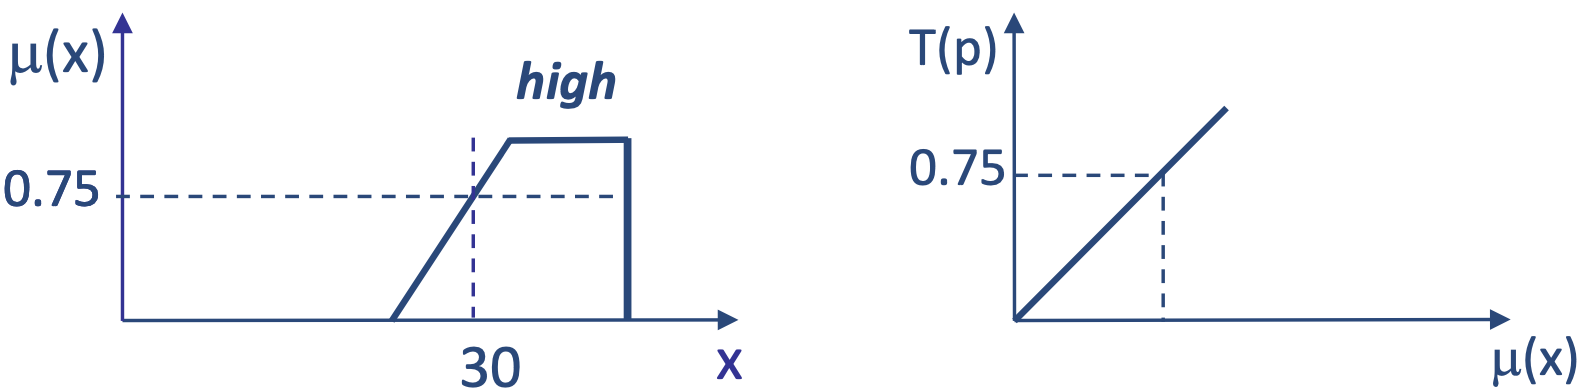
\includegraphics[width=0.5\linewidth]{images/temperature.png}
    \end{figure}
    Consequently, the truth value of the given proposition is 0.75.
\end{example}

It is also possible to express qualified, non-conditional propositions using the syntax "p: (X is F) is S", where:
\begin{itemize}
    \item S is a fuzzy truth qualifier.
    \item F is a fuzzy set.
    \item p is truth qualified.
\end{itemize}
\begin{example}
    Consider the conditional proposition "p: age of Tina is young is very true", where X represents age, F represents young, and S represents very true. 
    To determine the truth value of this proposition, we can refer to the graph of the membership function as shown below:
    \begin{figure}[H]
        \centering
        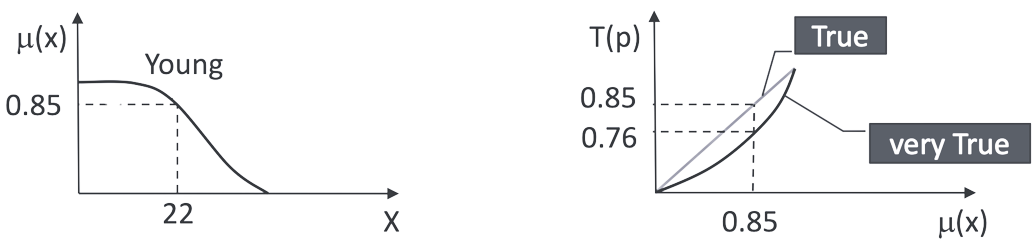
\includegraphics[width=0.75\linewidth]{images/age.png}
    \end{figure}
\end{example}

In fuzzy logic, fuzzy modifiers are employed to adjust the truth values of propositions. These modifiers can be categorized into two main types:
\begin{itemize}
    \item Strong ($m(a) \leq a \: \forall a \in [0 \dots 1]$): these modifiers strengthen the predicate, leading to a reduction in the truth value of the proposition.
    \item Weak($m(a) \geq a \: \forall a \in [0 \dots 1]$): these modifiers weaken the predicate, resulting in an increase in the truth value of the proposition.
\end{itemize}
The key properties of fuzzy modifiers include:
\begin{itemize}
    \item $m(0)=0$ and $m(1)=1$.
    \item $m$ is a continuous function. 
    \item If $m$ is a strong modifier, then $m^{-1}$ is a weak modifier, and vice versa.
    \item When combining another modifier $g$ with $m,$ and vice versa, the resulting composition is also a modifier. 
        If both $m$ and $g$ are strong (or weak), their composition is also strong (or weak).
\end{itemize}
\begin{example}
    The sentence "x is young" can be represented as "(x is young) is true". This sentence can be modified using fuzzy modifiers in the following ways:
    \begin{itemize}
        \item x is very young is true.
        \item x is young is very true.
        \item x is very young is very true.
    \end{itemize}
    Graphically, we can visualize the modified membership function as follows:
    \begin{figure}[H]
        \centering
        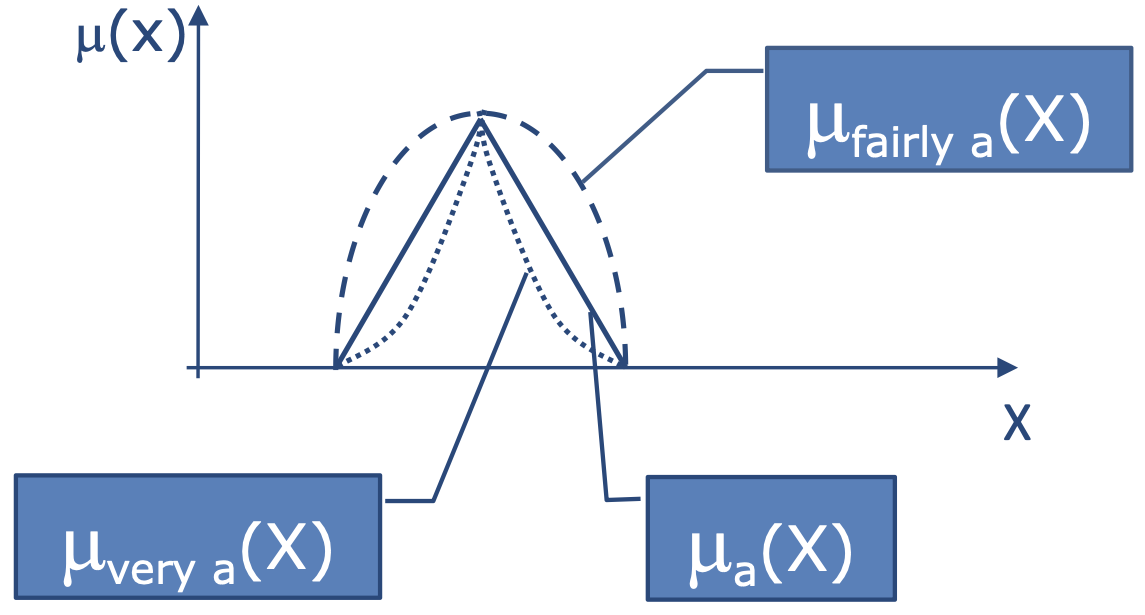
\includegraphics[width=0.4\linewidth]{images/modifiers.png}
    \end{figure}
    Here, we have:
    \begin{itemize}
        \item $\mu_{very \: a}(x)=\mu_a(x)^2$.
        \item $\mu_{fairly \: a}(x)=\mu_a(x)^{\dfrac{1}{2}}$.
    \end{itemize}
\end{example}